\section{Methods}
\label{mmf-sec:methods}

With the change from a variant-focused approach to a read-based method, our method  MisMatchFinder analysed ``mismatches`` of a read from the reference genome rather than a genomic locus. This \change{had the advantage of not requiring}{new approach did not require} a matched normal and could theoretically be used for virtually any sequencing data source like TAS, WES, WGS or \remove{even} RNA sequencing. However, it also meant that the error suppression methods, which are usually used by variant calling methods like read position ranks sum (RPRS) or strand bias, were not applicable. To solve the problem of high background noise, we developed multiple filtering steps, which are presented in the following sections.

\subsection{Mathematical concept}
\label{mmf-sec:concept}
A mismatch in this work was considered \remove{as} any position in an aligned read which did not show the same base as the reference at the aligned position. The mismatch inherited all the metrics of the read, such as mapping quality, base quality and read position. 

Ultimately, there were three sources of mismatches in a read\change{, which are}{:} somatic variants, germline variants and sequencing errors (\autoref{mmf-eq:1}).
\begin{equation}
n(mismatches) = n(somatic~var.) + n(germline~var.)  + n(seq.~ error)
\label{mmf-eq:1}
\end{equation}
\myequation[\ref{mmf-eq:1}]{MisMatchFinder: number of mismatches}

With the sequencing error being a function of the sequencing machine and chemistry, the error rate was assumed to be stable, almost constant, when using the same type of sequencing machine and chemistry \cite{Schirmer2016,Stoler2021}. We, therefore, reduced \autoref{mmf-eq:1} to
\begin{equation}
n(mismatches) = n(som.~var.) + n(germ.~var.)  + c_{seq.~err.}
\label{mmf-eq:2}
\end{equation}
\myequation[\ref{mmf-eq:2}]{MisMatchFinder: sequencing error}

Secondly, the number of germline variants was assumed to be approximately the same between two people \cite{Auton2015}, which again simplified \autoref{mmf-eq:2}:

\begin{equation}
n(mismatches) = n(som.~var.) + c_{germ.~var.} + c_{seq. err.}
\label{mmf-eq:3}
\end{equation}\myequation[\ref{mmf-eq:3}]{MisMatchFinder: germline variants}

Of course, \autoref{mmf-eq:3} was a crude estimate, and instead, the constants exhibited variability and were not real constants. To better approximate the inherent variableness of sequencing error and number of \add{the} germline variants, we instead used Gaussian distributions 

\begin{equation}
n(mismatches) = n(som.~var.) + \mathcal{N}(\mu_{germ.~var.}, \sigma_{germ.~var.}^{2}) + \mathcal{N}(\mu_{seq.~err.}, \sigma_{seq.~err.}^{2})
\label{mmf-eq:4}
\end{equation}
\myequation[\ref{mmf-eq:4}]{MisMatchFinder: number of mismatches with distributions}

However, both \Autoref{mmf-eq:3,mmf-eq:4} allowed the same conclusion, that with small enough values for either $c_{germ.~var}/c_{seq.~err.}$ or $\mu_{germ.~var}/\mu_{seq.~err.}$ and $\sigma_{germ.~var}/\sigma_{seq.~err.}$ respectively, there exists a linear correlation between the \change{amount}{number} of mismatches on a read and the somatic variants it contained:

\begin{equation}
n(mismatches) \sim n(som.~var.)
\label{mmf-eq:final}
\end{equation}
\myequation[\ref{mmf-eq:final}]{MisMatchFinder: number of mismatches correlation with somatic variants}

\add{As previously mentioned, the number of germline variants in a sample is orders of magnitudes higher than the number of somatic variants. Furthermore, the number of technical errors also out scales the number of somatic variants, which originally led to the development of variant calling methods. Therefore, the equations mentioned above are only valid after the filters we developed to reduce the impact of germline variants and technical errors substantially}

With the help of \autoref{mmf-eq:final}, we \change{were theoretically able to}{can} approximate tumour mutational burden and signatures from individual reads with MisMatchFinder. The method, therefore, was independent of read depth and required no matched normal sample for somatic variant calling.

\subsection{Data preprocessing}
As MisMatchFinder employs multiple internal measures to filter and process sequencing data, the steps used for preprocessing were minimal: The reads were  aligned to the GRCh38 reference genome (\autoref{intro-sec:mapping}). For optimal mapping and additional noise reduction, paired-end sequencing of at least 75 bp is required to ensure a few bases overlap on the standard fragment length of less than 155~bp of ctDNA (\autoref{intro-sec:ctDNA}). 

All datasets in this work were sequenced with 100~bp paired-end, aligned with BWA to GRCh38, and optical duplicates were marked with Picard unless further specified.

\subsection{Mismatch detection}
In contrast to conventional variant calling approaches, which find regions of interest through pileups (position-wise) and then realign reads in the surrounding area, to accurately estimate the most likely event that led to the observed haplotype (\autoref{intro-sec:variantcalling}), with MisMatchFinder we evaluated every individual read pair as a separate entity\change{ to}{. By analysing individual reads, we can} fully span the heterogeneity of all cells and their genetic background. The ``MD``- and ``CIGAR``-tags of \add{the preprocessed BAM file's} sequencing reads \remove{from the preprocessed BAM file} were used to reconstruct the sequence of the read and the positions where the read showed a different base than the reference. These potential mismatch sites were then filtered in multiple steps to reduce the impact of both germline variants \change{as well as}{and} sequencing errors, to ensure the assumptions of \autoref{mmf-sec:concept} held\remove{ true}.

\subsection{Filtering steps}
Apart from the standard filters, which most variant callers employ, like mapping quality (MQ) and base quality (BQ), which were used to ignore reads as well as read positions, respectively, the method also internally filters out common sequencing errors next to homopolymer regions \cite{Heydari2019}. While we set default cutoffs for optimal performance on our data (MQ=20, BQ=55, homopolyLength=5), the program allows \change{the user}{users} to adjust them to their liking.
This adjustment is also possible for both the region of interest (ROI) bed-file, which was used to restrict the analysis to only highly mappable regions of the genome (\autoref{ch-mmfAppendix:bedfiles}), \change{as well as for}{and} multiple other parameters. These include \add{the} minimum average base quality, minimum and maximum number of mismatches per read and fragment, and the minimum and maximum length of a fragment \cite{Hudecova2021}. If \remove{any of} these values were not within the specified range, the read was discarded from the analysis. No read flagged as secondary or duplicate was included in the analysis.

\subsection[Consensus reads]{Consensus reads - what happens when the sequencer isn't sure}
\label{mmf-sec:consensus}

When paired-end sequencing of ctDNA is analysed, the fraction of fragments where reads overlap is higher than with ``normal`` tissue-based sequencing due to the shorter fragment length of ctDNA (\autoref{intro-sec:ctDNA}). This overlap allowed a fragment internal consensus calculation by adjusting for differences between forward and reverse reads. In many variant calling methods, these differences are used by measuring the ``strand bias`` \cite{Guo2012, Saunders2012, GATKTeam2019} or ``strand balance probability`` \cite{Garrison2012} by looking at a specific locus and evaluating the discrepancy of all forward, and all reverse reads. As our method examined each read/fragment independently, th\change{e}{is} bias could not be calculated\change{, h}{. H}owever, \add{a consensus was generated }in the overlapping region of both reads\remove{, a consensus was generated}. If both reads agreed on the mismatch, the BQ of both reads were summed to emphasise the increased evidence for this variant. In contrast, if they disagreed, the \change{base of the higher quality}{higher quality base} was used, and its quality was decreased by half of the BQ of the lower quality base (\autoref{fig:mmf-consensus}~bottom). \add{This quality adjustment was taken from the samtools mpileup procedure and it is very conservative for mismatches and permissive for changes where both reads agree. This behaviour is intentionally chosen over other methods like FLASH }\cite{Magoc2011}\add{ and PEAR }\cite{Zhang2013}\add{ for a more restrictive analysis.} 

To further increase the stringency of the method, the user can also enable the \lq\emph{--strictOverlap}\rq\ option, which will only consider a mismatch if both reads agree with each other. As we were only interested in mismatches from the reference, all positions where both agree with the reference were irrelevant for the analysis and were discarded (\autoref{fig:mmf-consensus}~top). For the most stringent analysis, MisMatchFinder can additionally be configured to only use mismatches in the overlap part of a fragment (\lq\emph{--onlyOverlap}\rq), \change{which significantly reduced}{significantly reducing} the number of sequencing errors \remove{which were} retained in the final analysis (\autoref{mmf-sec:cleanSim}).

\begin{figure}[!ht]
\centering
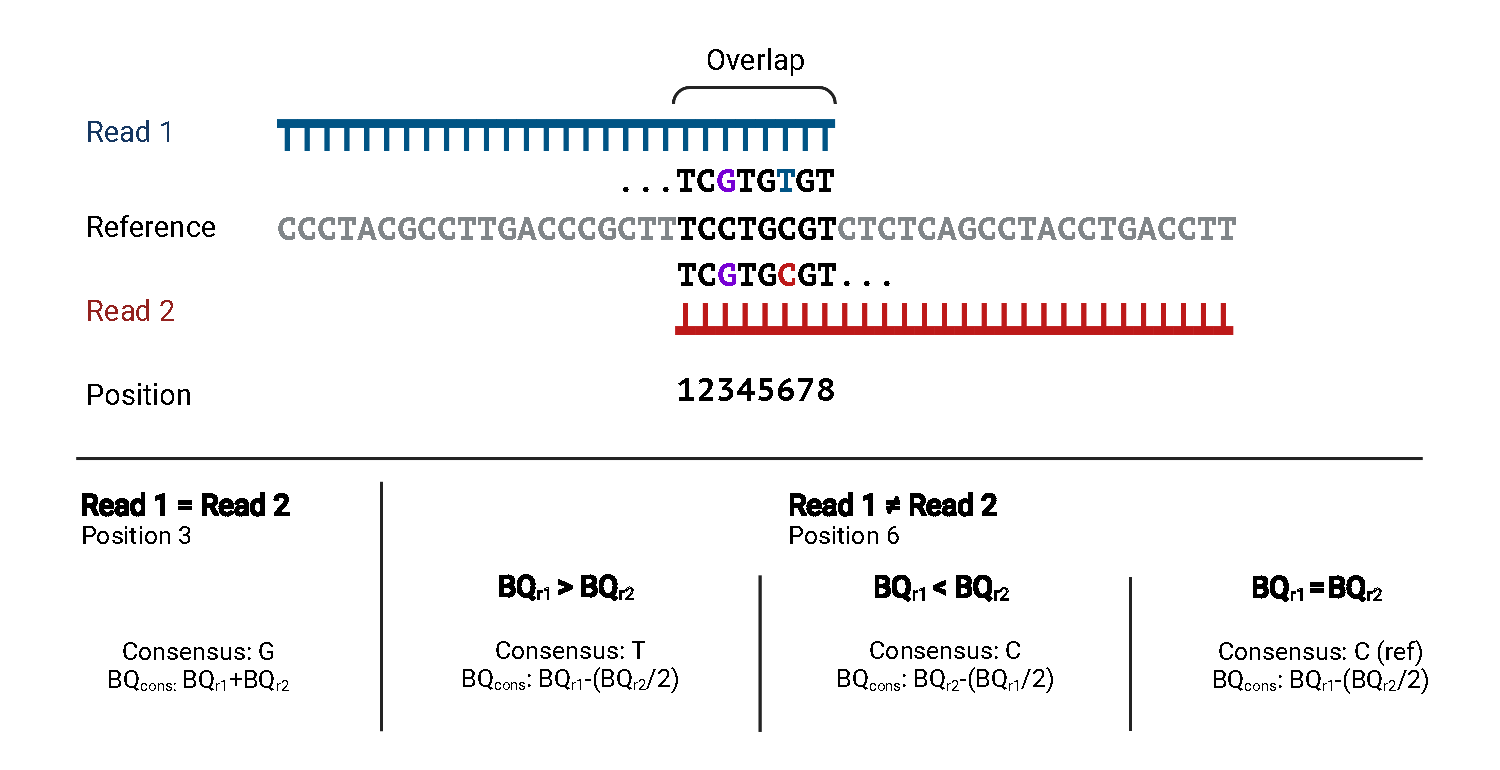
\includegraphics[width=.99\linewidth]{Figures/MisMatchFinder/ConsensusMethodMisMatchFinder.pdf}
\caption[Schematic of consensus computation method for overlapping reads]{Schematic of consensus computation method for overlapping reads in MisMatchFinder; Read 1 and Read 2 depict two overlapping paired end reads aligned to the reference sequence; Positions in the overlap are numbered for later referral; Read positions agreeing with the reference are coloured black, positions differing from the reference but agreeing in both reads are coloured purple (position 3) and differences between reads are coloured in the respective read colours (blue and red, position 6); Calculation for the resulting base quality (BQ$_{cons}$ for each possibility is shown as formulas)}\label{fig:mmf-consensus}
\end{figure}

This option, however, also reduced the available data by restricting the analysis to areas where reads were overlapping. Due to the fragment size distribution of ctDNA, a paired end sequencing with 100~bp read length will statistically,\remove{ in most cases} lead to an overlap of at least 45 nucleotides (\autoref{intro-sec:ctDNA}) and with 150~bp read length, most ctDNA fragments will be almost entirely covered by both reads. However\remove{, due to soft-clipping and incomplete alignment}, this number was lower in reality\add{ due to soft-clipping and incomplete alignment}.
In our tests, the restriction led to approximately 18 nucleotides (min:~14bp max:~25bp std.dev.:~1.45) being retained in the analysis out of 100. Nevertheless, this meant that with a read depth of 8-10x $\approx$80\% of the genome was covered by the overlap of at least one read pair.



\subsection[Germline filtering]{Germline filtering - exclusion of normal variation}
\label{mmf-sec:germline}

To further ensure the \autoref{mmf-sec:concept} assumption that the germline is a very small constant, we needed to remove as many mismatches as possible, \change{which originated}{originating} from germline variants. For this purpose, we built a custom zarr \cite{Miles2021} based storage system from the gnomAD database (v.3.1) \cite{Karczewski2020} using scikit-alel \cite{Miles2021a}.
An in-depth explanation of the generation \change{as well as}{and} a script for an end user can be found in \autoref{ch-mmfAppendix:germlineFilter}.

It allowed precise filtering of known germline variant sites from the analysis. The method enables the specification of an allele frequency cutoff, but as a default, all sites which were detected in any sample in gnomAD were filtered. We even included sites with low-quality variants in the database, as these were sites of sequencing or mapping complications, which most likely interfered with our analysis as well.


\subsection[Count normalisation]{Count normalisation}
\label{mmf-sec:countNorm}
After the filtering steps, all remaining mismatches were aggregated to oligo-nucleotide counts. With this step, we also classified directly neighbouring mismatches as DBS, which were counted as separate entities. SBS and DBS \remove{both} can be used to identify underlying biological mutational processes, but they have very different \add{associated} signatures \remove{associated with them }\cite{Alexandrov2020}.
 
The counts formed this way were influenced by the background frequency of their reference oligo-nucleotides in the analysed genomic region. As the frequencies of di- and tri-nucleotides are not uniformly distributed in the genome, the chance for a mismatch found in an ``AAA`` reference context is almost seven times higher than a mismatch in ``CGC`` (\autoref{A:mmf:tab:tricounts}, \autoref{A:mmf:tab:dicounts}). To reduce this bias towards high-frequency oligo-nucleotides, we implemented a count normalisation step.

First, the di- and tri-nucleotides in the analysed regions were counted using the reference without any black-listed or white-listed regions. These counts were then either \begin{enumerate*}[label={(\roman*)}]
 \item used to directly weight the observed mismatch counts, which led to a more uniform distribution of mismatches, or
 \item by building a fraction of observed oligo-nucleotides and the total counts in the genome
\end{enumerate*} (\autoref{A:mmf:tab:tricounts}, \autoref{A:mmf:tab:dicounts})\change{, the}{. This} weighting achieved an approximation of how the counts would have been distributed if the whole genome was analysed. These two options are available with \lq\emph{--normaliseCounts}\rq~ for \change{the approximation to}{approximating the} full genome. By \change{also}{additionally} adding \lq\emph{--flatNormalisation}\rq, only the observed counts are used for normalisation.

All analysis presented in this work was not normalised, as the white-listed regions used showed no significant difference in oligo-nucleotide abundance.

\subsection[Signature deconvolution]{Signature deconvolution - finding the original signal}
\label{mmf-sec:sigDeconv}
The deconvolution of the involved signatures from a known set of signatures is equivalent to finding the minimal distance between $m$ as the observed number of mismatches in each oligo-nucleotide context (a vector of length 96) and $\textbf{S}w$, where $\textbf{S}$ is the matrix of oligo-nucleotide defined contributions for each signature, resulting in a matrix of $96 \times k$ with $k$ being the number of known signatures. Lastly, $w$ is the vector of weights of each signature, which we aimed to estimate. 

\begin{align}
 \text{minimise:} & \quad (m - \textbf{S}w)^T(m - \textbf{S}w)
 = m^Tm - w^T\textbf{S}^Tm - m^T\textbf{S}w + w^T\textbf{S}^T\textbf{S}w \label{mmf-eq:optim1}\\
 \text{with:} & \quad \sum_j w_j = 1 \quad \text{and} \quad \boldsymbol{\forall} j ~ w_j \geq 0 \label{mmf-eq:requirements}
\end{align}
\myequation[\ref{mmf-eq:optim1}]{MisMatchFinder: optimisation for signature weights}
\myequation[\ref{mmf-eq:requirements}]{MisMatchFinder: optimisation function restrictions}

\autoref{mmf-eq:optim1} can then be written as 

\begin{equation}
\text{minimise:} \quad - m^T\textbf{S}w + \frac{1}{2}w^T\textbf{S}^T\textbf{S}w
\label{mmf-eq:optim2}
\end{equation}
\myequation[\ref{mmf-eq:optim2}]{MisMatchFinder: quadratic programming formula}

with the same restrictions as shown in \autoref{mmf-eq:requirements}. These equations and the idea to solve them with quadratic programming (QP) have been taken from \textcite{Lynch2016}, and the iterative linear models (ILM) solving approach was adapted from deconstructSigs \cite{Rosenthal2016}. Both methods were reimplemented in python in MisMatchFinder, using the quadprog package \cite{McGibbon2021} for QP and \change{a translation of}{translating} the R code of deconstructSigs for ILM.

MisMatchFinder allows the use of either QP or ILM, as they, in many cases, produce very similar results \cite{Lynch2016}. However, the default method is QP, even though ILM is the more interpretable and \remove{ more} parsimonious method\change{, b}{. B}ecause of the increased number of signatures, in the latest work by \textcite{Alexandrov2020}, ILM \change{did not resolve}{only resolved} the correct signatures if the signal was \remove{not }strong enough. QP, on the other hand, showed more stable solutions (\autoref{fig:mmf-ILMerror}).

\begin{figure}[!ht]
\centering
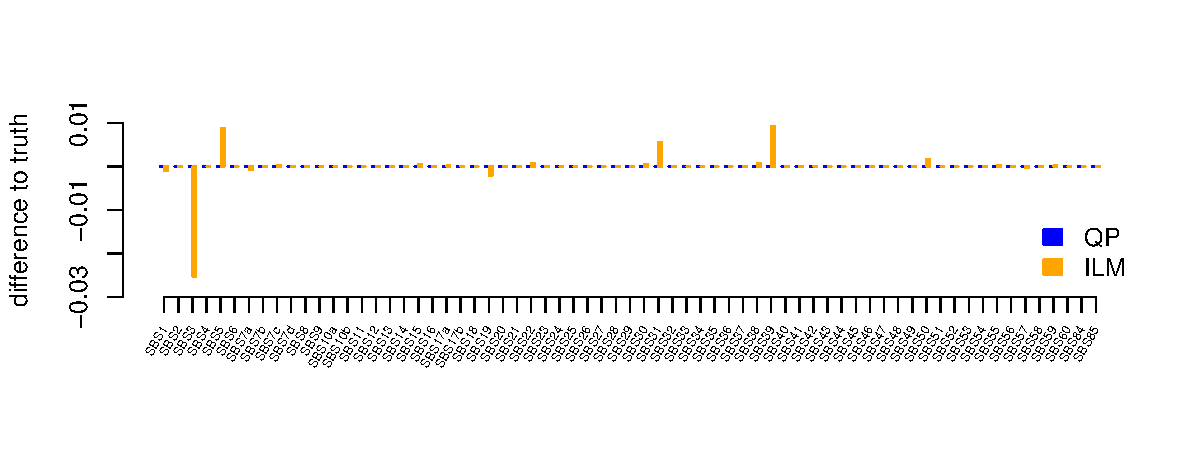
\includegraphics[width=.99\linewidth]{Figures/MisMatchFinder/lowInputSignalDeconv.pdf}
\caption[Distance of deconvolution methods from truth]{Distances of the estimated weights generated with ILM and QP from the true weight used as input; Truth is a synthetic count sample with (SBS1: 0.25; SBS3: 0.05; SBS5: 0.46; SBS7a: 0.1; SBS19: 0.03; SBS21: 0.01; SBS31: 0.08; SBS57: 0.02;)}\label{fig:mmf-ILMerror}
\end{figure}
 
The combinatorial problem in ILM, already shown by \textcite{Lynch2016}, was exacerbated  with ``wide`` signatures like SBS3 (\autoref{fig:sig7a}) and low signature contribution weights. As we were interested in analysing low tumour purity samples with low somatic signature signals from ctDNA, ILM was less sensitive in our test. Especially for SBS3, the \add{signature} contribution\remove{ of the signature} was only assigned by ILM with sufficient signal (15 and 20 mutations per megabase, respectively, for SBS7a and SBS3)\change{ where}{. In contrast,} QP allowed \remove{for }a more linear \add{signal} increase\remove{ in signal}, even at lower levels. On the other hand, ILM will assign an overall higher proportional weight than QP once the signal reaches a certain threshold (\autoref{fig:mmf-methodDifferences}). ILM was, therefore, better suited for high confidence signals but less effective for the more subtle differences we expected from ctDNA.

The deconvolution method could be an area for further optimisation by creating a custom deconvolution system adjusted for ctDNA detection and the signatures present.

\change{For the rest of this work, u}{U}nless specified differently, the results shown \add{for the rest of this work} were generated using the QP deconstruction method.



\subsection{Signature detection}
\label{mmf-sec:sigdetection}
Signature deconvolution with QP resulted in non-negative signature weights for almost all of the signatures \remove{when} using MisMatchFinder-derived counts\change{, h}{. H}owever, a positive signature did not necessarily indicate the activity of this process in a tumour capacity due to the normal somatic mutation background and germline residual signal (\autoref{mmf-sec:germlineArtifacts}). To enable \add{the} calling of significantly active signatures in samples, we developed a z-score-like system, which used the distribution of each signature weight in the healthy population as a background.

As the weight values after deconvolution were between 0 and 1 inclusive, with a high enrichment for 0 and 0-adjacent weights, we chose the beta distribution with probability density function (PDF, \autoref{eq:betaPDF}) with shape parameters $\alpha$ and $\beta$ and normalisation constant $\Beta$ to ensure the cumulative density function (CDF) sums up to 1. 
\begin{equation}
f(x; \alpha ,\beta)= \frac{1}{\Beta(\alpha, \beta)} x^{\alpha-1}(1-x)^{\beta-1}
\label{eq:betaPDF}
\end{equation}
\myequation[\ref{eq:betaPDF}]{Beta distribution probability density function}

To enable a z-score like estimation, we calculated the $\lambda$-quantile of the cumulative density function of the beta distribution (\autoref{eq:betaCDF}) for each patient $p$ samples signature weight $w_s(p)$ of signature $s$ with healthy sample fitted shape parameters $\alpha_s$ and $\beta_s$ per signature by solving  for $\lambda$ resulting in the inverse beta cumulative density function (\autoref{eq:invBetaCDF}). 

\begin{equation}
F(x; \alpha ,\beta) = \frac{\displaystyle\int_{0}^{x} t^{\alpha-1}(1-t)^{\beta-1} dt}{\Beta(\alpha, \beta)}
\label{eq:betaCDF} 
\end{equation}
\myequation[\ref{eq:betaCDF}]{Beta distribution cumulative density function}

\begin{equation}
x = F^{-1}(\lambda; \alpha ,\beta) = \left\{ x: F(x; \alpha, \beta) = \lambda \right\}
\label{eq:invBetaCDF} 
\end{equation}
\myequation[\ref{eq:invBetaCDF}]{Inverse beta distribution cumulative density function}


This allowed us to estimate how many healthy samples would have a signature weight less than the patient sample for the respective signature $s$ (\autoref{eq:sigCDFScore}). While we did not see significant downregulation of signatures from the background, the method could support both over- and under-re\-pre\-sentation analysis. Ten per cent of all samples were removed from both tails of the distribution of each signature before fitting the shape parameters to minimise the impact of outliers and instead fit the core distribution.

\begin{equation}
\forall s \in Signatures,\ \forall p \in Patients:\ \text{CDF-score}(s,p) := \frac{w_s(p)}{F^{-1}(\lambda; \alpha_s ,\beta_s)}
\label{eq:sigCDFScore}
\end{equation}
\myequation[\ref{eq:sigCDFScore}]{MisMatchFinder: CDF score calculation per signature and patient}

We used $\lambda = 0.99$ to calculate CDF scores for all signatures and assumed a CDF score of more than 2 to be significantly different.

This allowed the prioritisation of significantly changed signatures in the tumour samples with regard to our healthy background depending on the desired application. A higher CDF score cut off could increase specificity at the cost of sensitivity.

While most signature weights could be estimated very well with the moment matching estimation of fitdistrplus \cite{DelignetteMuller2015}, some signatures did not show an ideal fit. However, in these cases, the fit resulted in a wider distribution with higher theoretical quantiles than empirically observed, \change{which reduced}{reducing} the predictive power of the signature. These signatures also showed a double peak distribution indicative of a population sub-structure in the healthy population (\Autoref{A:fig:fittedDistsSBS3,A:fig:fittedDistsSBS17a} vs. \Autoref{A:fig:fittedDistsSBS12,A:fig:fittedDistsSBS46}).


\subsection{Tumour detection}
\label{mmf-sec:tumourdetection}

With the calling of ``active`` signatures in \autoref{mmf-sec:sigdetection}, we were subsequently interested in the classification of samples into ``healthy`` and perturbed (cancer) signature states. The classification as perturbed would allow a short-listing of samples for a more in-depth analysis with orthogonal validation.

For this purpose, we trained a glmnet classifier with the assigned signature weights vector of each sample with an $\alpha$ value of 0.7 due to the high correlation of the data.

The only other method which enables the classification of lcWGS of cfDNA into healthy and tumour (perturbed) samples was ichorCNA, which uses the copy number state of the sample to infer tumour purity  \cite{Adalsteinsson2017}. ichorCNA is currently considered the gold standard, and we used their default method \remove{as a reference} to compare our results\remove{ to}. Any sample with a tumour purity of $\geq$ 3\% was considered a positive and everything else a negative sample, as suggested by the ichorCNA developers.

The clinical status of disease was used as the ground truth for each sample. Every sample which was taken during a time when the patient had active disease was assigned the tumour class and every healthy individual the healthy class.
